\documentclass{article}
\usepackage[margin=0.5in]{geometry}
\usepackage{titlesec}
\usepackage{graphicx}
\usepackage{enumitem}
\usepackage{ifthen}
\usepackage{fancyhdr}
\usepackage{xcolor}

% -------- %
% SECTIONS %
% -------- %
\newcounter{problemnumber}\setcounter{problemnumber}{1}
\titlespacing\section{0pt}{10pt}{0pt}   % Spacing between Problems
\titlespacing\subsection{0pt}{5pt}{0pt} % Spacing between Parts
\newcommand{\problem}[1][-1]{
    \setcounter{partnumber}{1}
    \ifnum#1>0
        \setcounter{problemnumber}{#1}
    \fi
    \section*{Problem \arabic{problemnumber}}
    \stepcounter{problemnumber}
}

\newcounter{partnumber}\setcounter{partnumber}{1}
\newcommand{\ppart}[1][-1]{
    \ifnum#1>0
        \setcounter{partnumber}{#1}
    \fi
    \subsection*{Part \parttype{partnumber}}
    \stepcounter{partnumber}
}

\newenvironment{question}{
    \color{gray}\itshape
    \vspace{5pt}
    \begin{tabular}{|p{0.97\linewidth}}
}{
    \end{tabular}\\[5pt]
}



% ------------- %
% HEADER/FOOTER %
% ------------- %
\setlength\parindent{0pt}
\setlength\headheight{30pt}
\headsep=0.25in
\pagestyle{fancy}
\lhead{\ifthenelse{\thepage=1}
    {\textbf{Trevor Smith} \\ \textbf{\writeday}}
}
\chead{\ifthenelse{\thepage=1}
    {\textbf{\huge{HOMEWORK \hwnumber}}}
    {\textbf{\large{HOMEWORK \hwnumber}}}
}
\rhead{\ifthenelse{\thepage=1}
    {\textbf{{\course}} \\ \textbf{Professor {\prof}}}
}
\cfoot{\thepage}
\renewcommand\headrulewidth{0.4pt}
\renewcommand\footrulewidth{0.4pt}



% ---------- %
% PARAMETERS %
% ---------- %
% \PARTTYPE:
% \Alph   := "Part A, Part B,  ..."
% \alph   := "Part a, Part b,  ..."
% \arabic := "Part 1, Part 2,  ..."
% \Roman  := "Part I, Part II, ..."
\newcommand\parttype{\Roman}

% \COURSE:
\newcommand\course{PHYS 2303}

% \HWNUMBER
\newcommand\hwnumber{7}

% \SEMESTER
\newcommand\semester{Spring 2021}

% \PROF
\newcommand\prof{Skinnari}

% \WRITEDAY
% \today is date of compilation, replace if writing due date rather than write date
\newcommand\writeday{\today}



%  ------- %
% DOCUMENT %
% -------- %
\begin{document}
\problem
\begin{question}
An electron is in an (orbital) angular momentum state with l = 3.\\
(a) What is the length of this electron’s angular momentum vector?\\
(b) How many different possible z components can the angular momentum vector
have and what are these possible z components?\\
(c) What are the values of the angle that the angular momentum vector makes with the
z axis (this is the angle $\theta$ from class)? 
\end{question}
A)\\
$ L = \sqrt{l(l+1)}\bar{h} = 2 \sqrt{3} \bar{h} $ \\

B and C)\\
$cos\theta_m = \frac{m_l \bar{h}}{L}$ \\

\begin{table}[h]
	\begin{tabular}{l|lll}
		\textbf{$m_l$} & \textbf{$L_z$} & \textbf{$cos\theta_m$} & \textbf{$\theta$}(r) \\ \hline\hline
		3     &   $3\bar{h}$    &  $\sqrt{3}/2$ & $\pi/6$   \\ \hline
		2     &   $2\bar{h}$    &  $1/\sqrt{3}$ &  0.955  \\ \hline
		1     &    $1\bar{h}$   &  $1/(2\sqrt{3})$ & 1.277   \\ \hline
		0     &     $0$         &   0        & $\pi/2$    \\ \hline
		-1    &   $-1\bar{h}$   &  $-1/(2\sqrt{3})$ & 1.864   \\ \hline
		-2    &    $-2\bar{h}$  &  $-1/\sqrt{3}$ & 2.186   \\ \hline
		-3    &    $-3\bar{h}$  &  $-\sqrt{3}/2$ & $5\pi/6$   \\ \hline
	\end{tabular}
\end{table}

\newpage
\problem
\begin{question}
	Show that the ($n, l, m_l$) = (1, 0, 0) and (2, 0, 0) hydrogen atom wave functions (listed in
	Table 7.1 in the textbook) are indeed properly normalized. 
\end{question}
$$ P(r) dr = |R(r)|^2 r^2\ dr\ 
\int_0^\pi |\Theta(\theta)|^2\ sin(\theta)\ d\theta\ 
\int_0^{2\pi} |\Phi(\phi)|^2\ d\phi $$

$$ 1 = \int_0^\infty |R(r)|^2 r^2\ dr\ 
\int_0^\pi |\Theta(\theta)|^2\ sin(\theta)\ d\theta\ 
\int_0^{2\pi} |\Phi(\phi)|^2\ d\phi $$

For (1, 0, 0): \\
$$ \int_0^\pi |\Theta(\theta)|^2 sin(\theta) dr 
= \int_0^\pi \left|\frac{1}{\sqrt{2}}\right|^2 sin(\theta) dr $$
$$ = \frac{1}{2} (-cos(\pi) - -cos(0)) = 1/2 \cdot (-(-1) - (-1)) =  1 $$

$$ \int_0^{2\pi} \left|\Phi(\phi)\right|^2\ d\phi 
 = \int_0^{2\pi} \left|\frac{1}{\sqrt{2\pi}}\right|^2\ d\phi 
 = \frac{1}{2\pi} (2\pi - 0) = 1 $$

$$ 1 = \int_0^\infty |R(r)|^2 r^2\ dr $$
$$ 1 = \int_0^\infty \left|\frac{2}{a_0^{3/2}}e^{-r/a_0}\right|^2 r^2\ dr $$
$$ 1 = \frac{4}{a_0^{3}} \int_0^\infty 
e^{-2r/a_0} r^2\ dr $$

$$ = \frac{4}{a_0^{3}} 
\left( 
-e^{-2/a_0 \cdot r} 
\frac{(2/a_0)^2r^2 + 2(2/a_0)r + 2}
{(2/a_0)^3} 
\right)^\infty_0 $$


$$ =
\left( 
-e^{-2/a_0 \cdot r} 
\frac{4/a_0^2r^2 + 4/a_0r + 2}
{2} 
\right)^\infty_0 $$

The exponential grows faster than the numerator, so the evaluation of the limit as r approaches infinity is 0.

$$ 1 = e^{-2/a_0 \cdot r} 
\frac{4/a_0^2r^2 + 4/a_0r + 2}
{2} \ where\ r=0 $$


$$ 1 = 1 \cdot 
\frac{0 + 0 + 2}
{2} $$

The probability density equation is normalized properly. \\
\\

\newpage
For (2, 0, 0):\\
The equations for $\Theta$ and $\Phi$ are both the same, which means they end up being 1 again after integrating.

$$ 1 = \int_0^\infty |R(r)|^2 r^2\ dr $$
$$ 1 = \int_0^\infty 
\left|\frac{1}{(2a_0)^{3/2}}
	\left(2 - \frac{r}{a_0} \right) 
	e^{-r/(2a_0)} 
\right|^2 r^2\ dr $$

$$ 1 = \frac{1}{(2a_0)^{3}} \int_0^\infty 
\left(
	\left(4 - 4\frac{r}{a_0} + \frac{r^2}{a_0^2} \right) 
	e^{-r/a_0} 
\right) r^2\ dr $$

$$ 1 = \frac{1}{8a_0^{3}} \left[
\int_0^\infty 4r^2 e^{-r/a_0} dr
-
\int_0^\infty 4\frac{r^3}{a_0} e^{-r/a_0} dr
+
\int_0^\infty \frac{r^4}{a_0^2} e^{-r/a_0} dr
\right] $$

We can remember that the laplace transform of $r^n e^{-r} = \frac{n!}{c^6}$.

$$ 1 = \frac{1}{8a_0^{3}} \left[
4 \cdot 2! \cdot a_0^3
-
\frac{4}{a_0} \cdot 3! \cdot a_0^4
+
\frac{1}{a_0^2}4! \cdot a_0^5
\right] $$

$$ 1 = \frac{1}{8a_0^{3}} \left[
8 \cdot a_0^3
-
24 \cdot a_0^3
+
24 \cdot a_0^3
\right] $$

$$ 1 = \frac{1}{8} \left[
8 - 24 + 24
\right] $$

This function is also normalized properly.






\newpage
\problem
\begin{question}
Consider the radial probability density for the hydrogen atom wave functions. If n = 2
and l = 0, for what value of the radius (r) does the radial probability density have its
maximum values? 
\end{question}

$$ P(r) = |R(r)|^2 r^2\ dr $$
$$ P(r) = 
\left|\frac{1}{(2a_0)^{3/2}}
	\left(2 - \frac{r}{a_0} \right) 
	e^{-r/(2a_0)} 
\right|^2 r^2\ dr $$
From the previous problem. We'll just trim off the constants since they won't matter here.\\

$$ P(r) = 
\left(2r - \frac{r^2}{a_0} \right)^2
e^{-r/a_0} $$

$$ P(r) = 
\left(4r^2 - 4\frac{r^3}{a_0} + \frac{r^4}{a_0^2} \right)
e^{-r/a_0} $$

$$ \frac{dP}{dr} = 
e^{-r/a_0}(4r^2)(-1/a_0) + (8r)e^{-r/a_0} -
e^{-r/a_0}(4r^3/a_0)(-1/a_0) + (-12r^2/a_0)e^{-r/a_0} +
e^{-r/a_0}(r^4/a_0^2)(-1/a_0) + (4r^3/a_0^2)e^{-r/a_0}
$$

$$ \frac{dP}{dr} = 
e^{-r/a_0}
\left(
	(-4r^2/a_0) + (8r) +
	(4r^3/a_0^2) + (-12r^2/a_0) +
	(-r^4/a_0^3) + (4r^3/a_0^2)
\right)
$$

$$ \frac{dP}{dr} = 
e^{-r/a_0}
r\left(
	8 +
	-16/a_0r +
	8/a_0^2r^2
	-1/a_0^3r^3
\right)
$$
We did the derivative by hand, but we'll need to use wolfram to solve the 4th order polynomial equation for the max that we're looking for. We end up getting $\sqrt{5}a_0 + 3a_0$.


\newpage
\problem
\begin{question}
Now instead consider the angular probability density for the hydrogen atom wave
functions. Find the directions in space where the angular probability density for the
l = 2, m = 0 electron in hydrogen has its maxima and minima?
Hint: Consider dP/d$\theta$ as in example 7.7 in the textbook. 
\end{question}

$$ P(\theta, \phi) = |\Theta(\theta)\Phi(\phi)|^2 = \left|\sqrt{\frac{5}{8}}(3cos^2\theta-1)\frac{1}{\sqrt{2\pi}}\right|^2 $$
$$ P(\theta, \phi) = \frac{5}{8}(3cos^2\theta-1)^2\frac{1}{2\pi} $$
$$ P(\theta, \phi) =
\frac{5}{15\pi}\left(\frac{3}{2}(1 + cos2\theta)-1\right)^2 $$
$$ P(\theta, \phi) =
\frac{5}{16\pi}\left(\frac{3}{2}cos2\theta + 1/2\right)^2 $$

$$ \frac{dP}{d\theta} =
\frac{5}{8\pi} \left(\frac{3}{2}cos2\theta + 1/2 \right) (-3sin2\theta)
$$

$$ \frac{dP}{d\theta} =
\frac{5}{8\pi} \left(\frac{3}{2}cos2\theta + 1/2 \right) (-3sin2\theta)
$$
\smallskip
Zeroes occur where 
$$ \frac{3}{2} cos2\theta = -1/2 $$
$$ cos2\theta = -1/3 $$
Theta = 0.955 \\
And
$$ sin2\theta = 0 $$
Theta = 0. \\


We can look at the second derivative to determine which is maxima/minima.


$$ \frac{d^2P}{d\theta^2} =
\frac{5}{8\pi} \left(
\frac{3}{2}cos2\theta(-6cos2\theta)
+ (-3sin2\theta)(3/2 cos2\theta)
+ 1/2 (-6cos2\theta) \right) $$

We can tell from a cursory glance that the function is concave up at $\theta = 0.955 $ and concave down at $\theta = 0$, meaning the former is the min and the latter is the max. Just kidding, I plugged it into wolfram after doing the second derivative by hand.



\newpage
\problem
\begin{question}
For a hydrogen atom in the (3, 2, 0) state: \\
(a) Show that the wave function from Table 7.1 is properly normalized. \\
(b) What is the most likely radius of the electron? How does the result compare with
what the Bohr' model predicts? \\
(c) Calculate the average value of the electron’s potential energy. How does it compare
with the corresponding result from the Bohr model? 
\end{question}
A) \\

$$ P(r) dr = |R(r)|^2 r^2\ dr\ 
\int_0^\pi |\Theta(\theta)|^2\ sin(\theta)\ d\theta\ 
\int_0^{2\pi} |\Phi(\phi)|^2\ d\phi $$

$$ 1 = \int_0^\infty 
\left|\frac{4}{27\sqrt{10}(3a_0)^{3/2}}\frac{r^2}{a_0^2} e^{-r/(3a_0)}\right|
^2 r^2\ dr\ 
\cdot \int_0^\pi 
\left|\sqrt{\frac{5}{8}}(3cos^2\theta-1)\right|^2\ 
sin(\theta)\ d\theta\ 
\cdot \int_0^{2\pi} 
\left| \frac{1}{\sqrt{2\pi}} \right|
^2\ d\phi $$
We already know the Phi term is normalized. Looking at the theta term first:

$$ \int_0^\pi 
\left|\sqrt{\frac{5}{8}}(3cos^2\theta-1)\right|^2\ 
sin(\theta)\ d\theta\ $$

$$ \frac{5}{8} \int_0^\pi 
\left(3cos^2\theta-1\right)^2\ 
sin(\theta)\ d\theta\ $$

Where $u = \sqrt{3}cos\theta$, $\frac{du}{-\sqrt{3}} = sin\theta\ d\theta$ \\
And $\sqrt{3} = \sqrt{3}cos(0), -\sqrt{3} = \sqrt{3}cos(\pi)$ \\

$$ \frac{5}{8\sqrt{3}} \int_{-\sqrt{3}}^{\sqrt{3}}
\left(u^4 - 2u^2 + 1\right) du
$$

$$ \frac{5}{8\sqrt{3}} 
\left(1/5 u^5 - 2/3 u^3 + u\right)_{-\sqrt{3}}^{\sqrt{3}}
$$

Function is even
$$ \frac{10}{8\sqrt{3}} 
\left((1/5) 9\sqrt{3} - (2/3) 3\sqrt{3} + \sqrt{3}\right)
$$

$$ \frac{5}{4} 
\left(9/5 - 2 + 1\right)
$$

$$ \frac{5}{4} 
\left(9/5 - 5/5\right)
$$

The theta one is equal to 1. \\

$$ 1 = \int_0^\infty 
\left|\frac{4}{27\sqrt{10}(3a_0)^{3/2}}\frac{r^2}{a_0^2} e^{-r/(3a_0)}\right|
^2 r^2\ dr\ 
$$

$$ \frac{16}{27^2 \cdot 10(3a_0)^{3}} \int_0^\infty 
\left|e^{-r/(3a_0)}\right|
^2 \frac{r^4}{a_0^4} r^2\ dr\ 
$$

$3^3 = 27$ \\
$$ \frac{16}{27^3 \cdot 10(a_0)^{7}}
\int_0^\infty 
e^{-r\frac{2}{3a_0}}
r^6\ dr\ 
$$

\newpage
$c = \frac{2}{3a_0}, c^7 = \frac{2^7}{3^7a_0^7}$

$$ \frac{16}{27^3 \cdot 10(a_0)^{7}}
\left[
	\frac{e^{-rc}}{c}
	\left(\frac{c^6r^6 + 6c^5r^5 + 30c^4r^4 + 120c^3r^3 + 360c^2r^2 + 720cr + 720}{c^6}
\right)
\right]^\infty_0
$$

$27^3 = 3^73^2,\ 16 = 2^4$
$$ \frac{1}{3^2 2^4 \cdot 5}
\left[
	e^{-rc}
	\left(c^6r^6 + 6c^5r^5 + 30c^4r^4 + 120c^3r^3 + 360c^2r^2 + 720cr + 720
\right)
\right]^\infty_0
$$

At r = infinity, the integral evaluates to zero as the exponent rises faster than any polynomial.  \\
At r = 0, the exponent evaluates to 1 and every r term evaluates to zero. This leaves, after simplyfing the fraction at the beginning of the expression:
$$ \frac{1}{720} \left[720\right] = 1 $$

B)\\
We already verified that the integrals across Theta and Phi are 1. 
$$ P(r) = 
\left|\frac{4}{27\sqrt{10}(3a_0)^{3/2}}\frac{r^2}{a_0^2} e^{-r/(3a_0)}\right|
^2 r^2\ dr\ 
$$

$$ P(r) =  \frac{16}{27^3 \cdot 10(a_0)^{7}}
e^{-r\frac{2}{3a_0}}
r^6\ dr\ 
$$

$$ \frac{dP}{dr} =  \frac{16}{27^3 \cdot 10(a_0)^{7}}
\left(
	\frac{-2}{3a_0} e^{-r\frac{2}{3a_0}}
	r^6\ dr\ 
	+
	\frac{-2}{3a_0} e^{-r\frac{2}{3a_0}}
	r^6\ dr\ 
\right)
$$


$$ \frac{dP}{dr} =  \frac{16}{27^3 \cdot 10(a_0)^{7}} \cdot
r^5 \cdot e^{-r\frac{2}{3a_0}}\left(
	\frac{-2}{3a_0} 
	r
	+
	6
\right)
$$

We can see that there are zeros at infinity, 0, and $r = 9a_0$. This matches Bohr's prediction of $n^2 a_0$.

C)\\
$$ U(r) = -\frac{e^2}{4\pi\epsilon_0} \cdot \frac{1}{r} $$

$$ P(r) =  \frac{16}{27^3 \cdot 10(a_0)^{7}}
e^{-r\frac{2}{3a_0}}
r^6\ dr\ 
$$

$$ <U> = \int_0^\infty U(r) P(r) dr 
=  \int_0^\infty -\frac{e^2}{4\pi\epsilon_0} \cdot \frac{1}{r} 
 \frac{16}{27^3 \cdot 10(a_0)^{7}}
e^{-r\frac{2}{3a_0}}
r^6\ dr\ 
$$

$$ <U> 
= \frac{2^4}{3^9 \cdot 10(a_0)^{7}} 
\frac{-e^2}{4\pi\epsilon_0} 
\int_0^\infty 
e^{-r\frac{2}{3a_0}}
r^5\ dr\ 
$$

$$ c = \frac{2}{3a_0} $$

$$ <U> 
= \frac{c^7}{8}\frac{1}{90} 
\frac{-e^2}{4\pi\epsilon_0} 
\int_0^\infty 
e^{-rc}
r^5\ dr\ 
$$

$$ <U> 
= \frac{c^7}{8}
\frac{-e^2}{360 \pi\epsilon_0} 
\left[
	e^{-rc}\left(
		\frac{c^5r^5 + 5c^4r^4 + 20c^3r^3 + 60c^2r^2 + 120cr + 120}{c^6}
	\right)
\right]^\infty_0
$$

The integral is zero at infinity, and each r term is zero at zero.

$$ <U> 
= \frac{c^7}{8}
\frac{-e^2}{360 \pi\epsilon_0} 
\frac{120}{c^6}
$$

$$ <U> 
= \frac{c}{8}
\frac{-e^2}{3 \pi\epsilon_0} 
$$

$$ <U> 
= \frac{1}{36a_0}
\frac{-e^2}{\pi\epsilon_0} 
$$

This matches the classical prediction of $U = \frac{-e^2}{4\pi\epsilon_0 (9a_0)}$

\newpage
\problem
\begin{question}
Explain why each of the following sets of quantum numbers ($n, l, m_l, m_s$) is not
permitted for hydrogen: \\
(a) (2, 2, -1, +1/2) \\
(b) (3, 1, +2, -1/2) \\
(c) (4, 1, +1, -3/2) \\
(d) (2, -1, +1, +1/2) 
\end{question}
\begin{enumerate}[label=\Alph*]
	\item The maximum absolute value of $l$ is $n-1$
	\item The maximum absolute value of $m_l$ is $l$
	\item Electrons cannot have 3/2 spin
	\item There's no such thing as negative $l$ values
\end{enumerate}

\problem
\begin{question}
(a) A hydrogen atom is in an excited 5g state, from which it makes a series of transitions
by emitting photons, ending in the 1s state. Show, on a diagram similar to Figure 7.19
from the textbook, the sequence of transitions that can occur? \\
(b) Repeat part (a) if the atom instead begins in the 5d state? 
\end{question}

A) \\
\begin{figure}[h!]
	\centering
	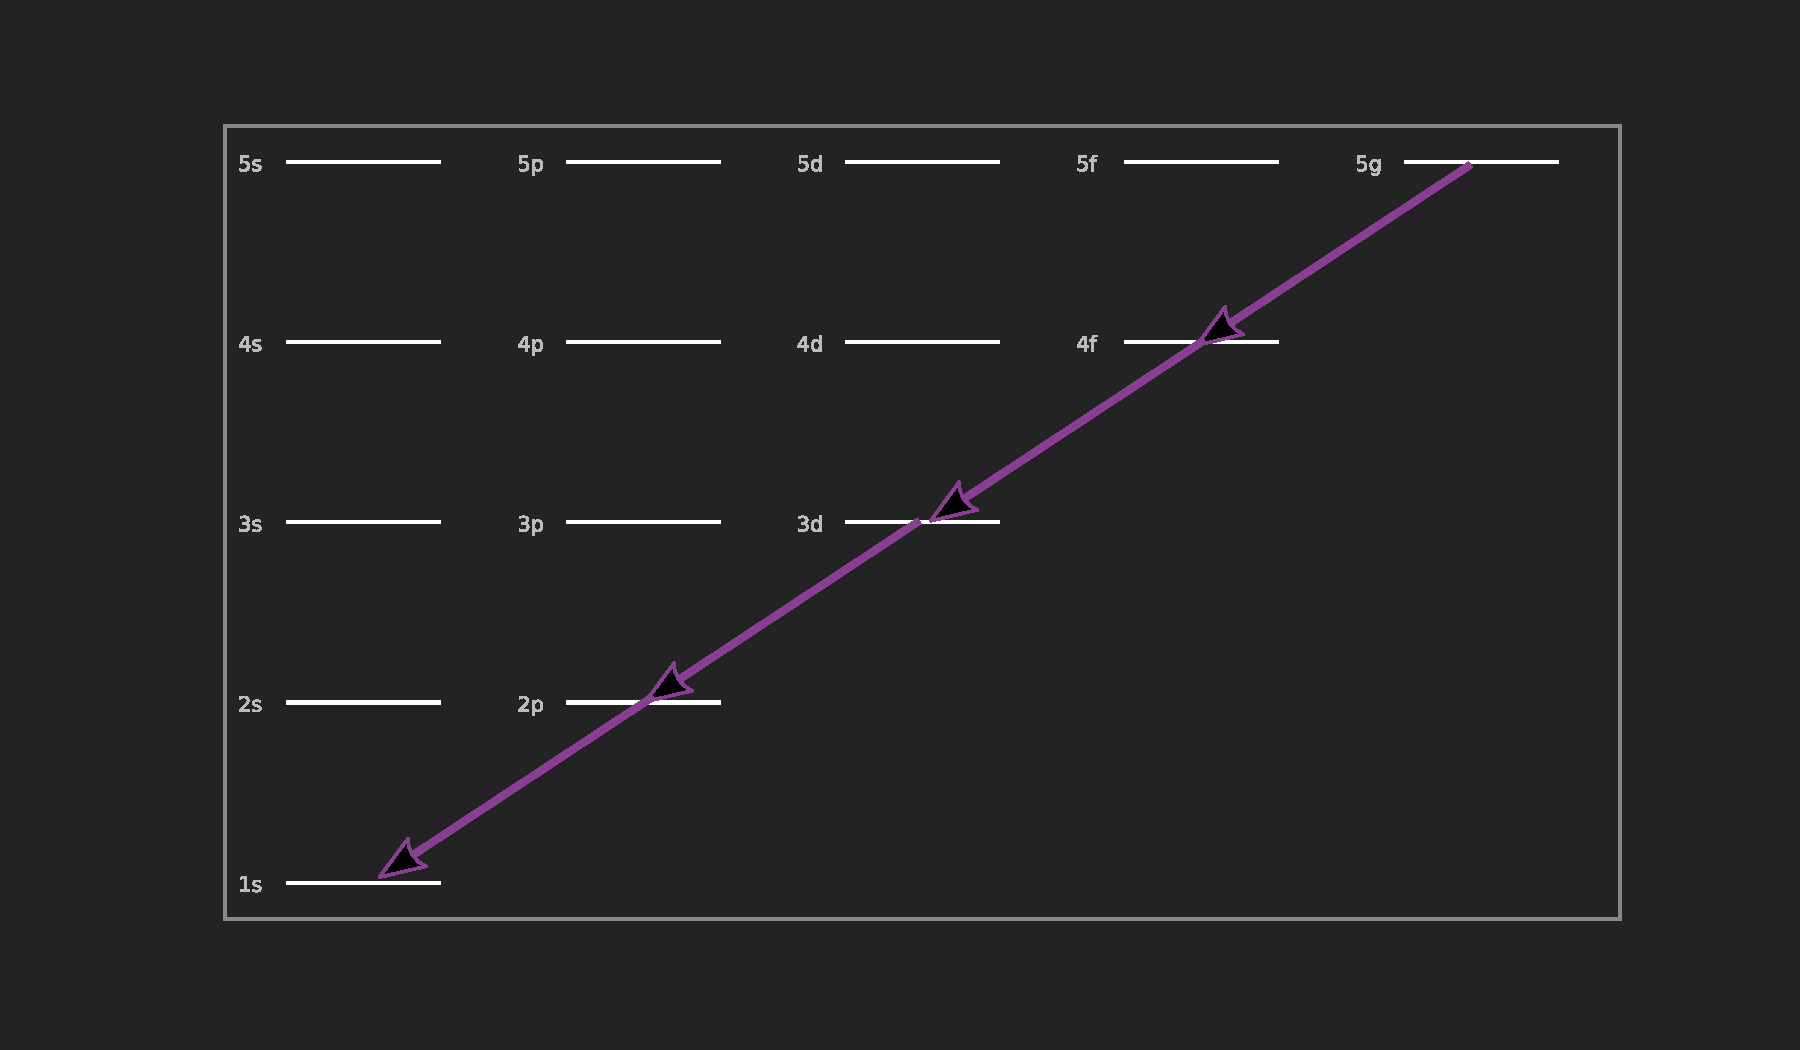
\includegraphics[width=1\linewidth]{./7a.pdf}
	\caption{}
\end{figure}

\newpage
B)\\
\begin{figure}[h!]
	\centering
	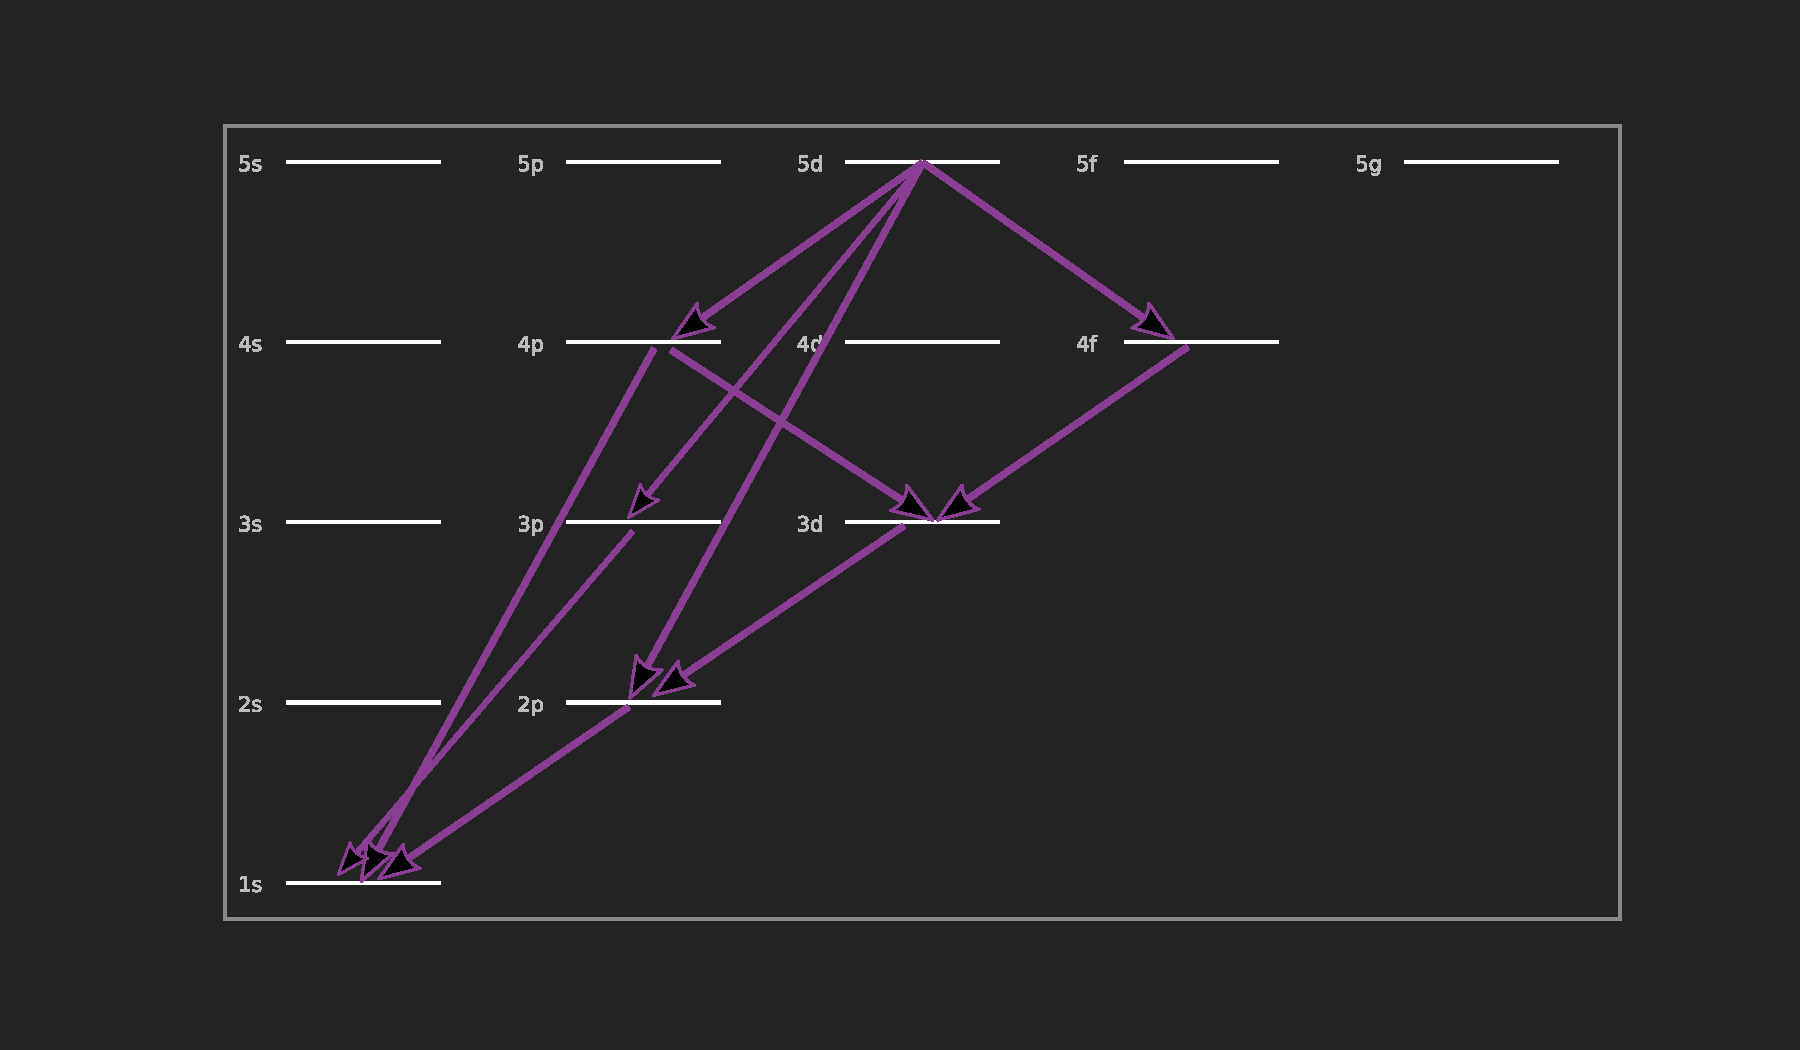
\includegraphics[width=1\linewidth]{7b.pdf}
	\caption{}
\end{figure}
\end{document}
